\documentclass[usletter, 12pt]{article}
\usepackage{amsmath}
\usepackage{enumitem}
\usepackage{graphicx}
\graphicspath{ {images/} }


\begin{document}


\begin{enumerate}[leftmargin=0em, label=\textbf{\arabic*}.]
  \setcounter{enumi}{2} % remove this if you want to add other solutions 


\item \textbf{Solution}: \vspace{3em}
  \noindent The equation of the orbit is
  \begin{equation}
    \frac{\alpha}{r} = 1+\varepsilon\cos(\phi)
  \end{equation}
  assuming without loss of generality that $\phi_0=0$. Here
  $\alpha=\displaystyle{\frac{\ell^2}{\mu k}}$ and $\varepsilon =
  \displaystyle{\sqrt{1+\frac{2E\ell^2}{mk^2}}}$. Therefore, the radial distance
  $r$ can vary from the maximum value $\displaystyle\frac{\alpha}{(1-\varepsilon)}$ to the minimum
  value $\displaystyle\frac{\alpha}{(1+\varepsilon)}$. \\

  \noindent The angular velocity of the particle is given by
  \begin{equation}
    \omega = \dot{\phi} = \frac{\ell}{\mu r^2}
  \end{equation}
  Thus, the maximum and minimum values of $\omega$ become,
  \begin{equation}
    \begin{cases}
      \omega_{\text{max}} = \displaystyle\frac{\ell}{\mu r_{\text{min}}^2} = \displaystyle\frac{\ell}{\mu\left[\frac{\alpha}{1+\varepsilon} \right]^2} \\ \\
      \omega_{\text{min}} = \displaystyle\frac{\ell}{\mu r_{\text{max}}^2} = \displaystyle\frac{\ell}{\mu\left[\frac{\alpha}{1-\varepsilon} \right]^2} 
    \end{cases}
  \end{equation}
  So that the ratio of the two is,
  \begin{equation}
    \frac{\omega_{\text{max}}}{\omega_{\text{min}}} = \left(  \frac{1+\varepsilon}{1-\varepsilon}\right)^2 \equiv n
  \end{equation}
  From which we have
  \begin{equation}
    \varepsilon = \frac{\sqrt{n}-1}{\sqrt{n}+1}
  \end{equation}
\newpage





\item \textbf{Solution}:\vspace{3em}
  \noindent The force $f(r)=-k/r^3$ can be easily integrated to find the
  corresponding central potential
  \begin{equation}
    V(r) = -\frac{k}{2r^2}
  \end{equation}
  The corresponding effective potential is formed by adding in the kinetic
  energy due to rotations. That is,
  \begin{equation}
    V_\text{eff}(r) = \frac{\ell^2}{2\mu r^2}-\frac{k}{2r^2}
  \end{equation}
  The equation for the shape of an orbit is
  \begin{equation}
    \frac{d^2u}{d\phi^2} + u = -\frac{\mu}{\ell^2u^2}\left(-ku^3 \right)
  \end{equation}
  or,
  \begin{equation}
    \frac{d^2u}{d\phi^2} + \left[ 1 - \frac{\mu k}{\ell^2} \right]u = 0
  \end{equation}
  Let us consider the motion of various values of $\ell$.

  
  \begin{enumerate}[leftmargin=2em, label=(\textbf{\alph*})]
  \item $\ell^2=\mu k$: \\
    \noindent In this case, the effective potential vanishes and the orbit
    equation becomes
    \begin{equation}
      \frac{d^2u}{d\phi^2}=0
    \end{equation}
    which leads to orbits of the form
    \begin{equation}
      u = \frac{1}{r} = A\phi + B
    \end{equation}
    so that the particle spirals towards the force center.\\

  \item $\ell^2>\mu k$:
    \noindent In this case the effective potential is positive and decreases
    monotonically with increasing $r$. For any value of the total energy $E$, the
    particle will approach the force center and will undergo a reversal of
    motion at $r=r_0$; the particle will then proceed again to an infinite
    distance. This is illustrated in the following sketch
    \begin{figure}[!hbt]
      \centering
      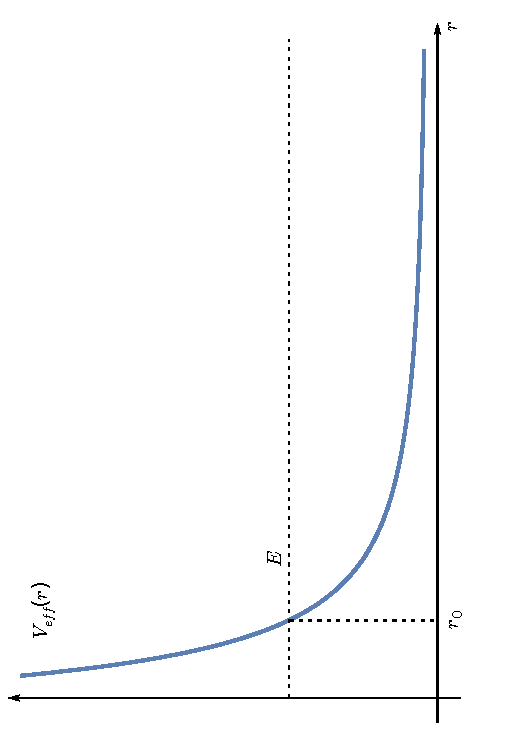
\includegraphics[width=0.7\columnwidth, angle=-90]{effective_potential_1.pdf}
    \end{figure}

    Setting $1-\mu k/\ell^2 = \beta^2 > 0$, then the differential equation
    becomes
    \begin{equation}
      \frac{d^2u}{d\phi^2}+\beta^2u = 0
    \end{equation}
    with the solution
    \begin{equation}
      u(\phi) = \frac{1}{r} = A\cos\left(\beta\phi -\delta\right)
    \end{equation}
    Since the minimum value of $u$ is zero, this solution corresponds to
    unbounded motion, as expected from the form of the effective
    $V_{\text{eff}}(r)$.\\ 

  \item $\ell^2<\mu k$:
   \noindent For this case we set $\mu k/\ell^2-1=G^2>0$, and the orbit equation
   becomes
   \begin{equation}
     \frac{d^2u}{d\phi^2} - G^2u = 0
   \end{equation}
   which leads to
   \begin{equation}
     u(\phi) = \frac{1}{r} = A\cosh(G\phi-\delta)
   \end{equation}
   so that the particle spirals in towards the force center.
  \end{enumerate}
  
\end{enumerate}


\end{document}

